latex: https://www.overleaf.com/

\documentclass{article}
\usepackage[utf8]{inputenc}
\usepackage{graphicx}

\title{TP Redes 5to Informática}
\author{Maite Lukasiunas, Marko Martín, Celeste Papalato }

\begin{document}

\maketitle

\section{SWITCH}

\text{\setlength{\parskip}{4mm}Un SWITCH es un equipo de interconexión utilizado para conectar equipos de red, formando las redes de área local LAN. El SWITCH es el elemento central de la topología en la red.}

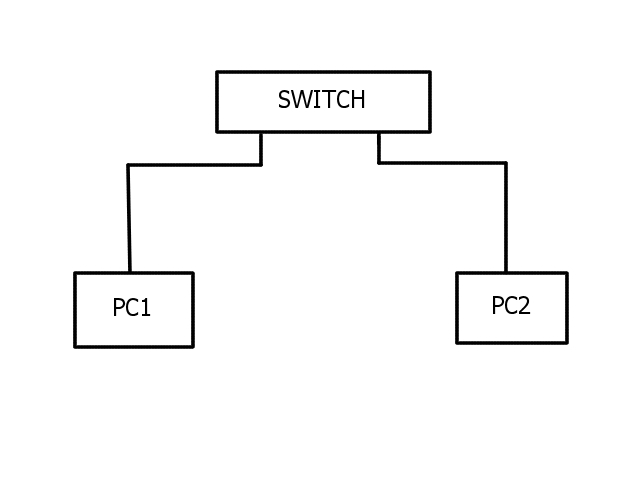
\includegraphics[width=\textwidth]{SWITCH.jpg}

\textit{Topología}:

PC1[0]=”A”

PC2[0]=”B”

SWITCH[0]=”A”

SWITCH[1]=”B”

\text{\setlength{\parskip}{10mm}\textbf{En PC1}:}

\text{\setlength{\parskip}{4mm}
//Activamos la placa de red:
}

ifconfig eth0 192.168.0.1 up


\text{\setlength{\parskip}{4mm}\textbf{En PC2}: 

//Activamos la placa de red:
}

ifconfig eth0 192.168.0.2 up

\text{\setlength{\parskip}{4mm}\textbf{En SWITCH}:

//Activamos las placas de red:
}

ifconfig eth0 up

ifconfig eth1 up

\text{\setlength{\parskip}{4mm}
//Creamos un puente entre las placas de ethernet:
}

brctl add br0

\text{\setlength{\parskip}{4mm}
//Añadimos la primer placa:
}

brctl addif br0 eth0

\text{\setlength{\parskip}{4mm}
//Añadimos la segunda placa:
}

brctl addif br0 eth1

\text{\setlength{\parskip}{4mm}
//Activamos el puente:
}

ifconfig br0 up

\text{\setlength{\parskip}{10mm}Ahora el switch podrá enviar los paquetes de las 2 PC debido a que conectamos las placas de ethernet con un \textit{bridge}. }

\section{VLAN}

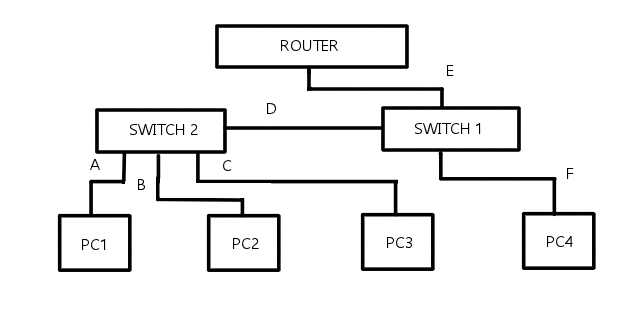
\includegraphics[width=\textwidth]{VLAN.jpg}

\textit{Topología}:

PC1[0]="A"

PC2[0]="B"

PC3[0]="C"

PC4[0]="F"


SW1[0]="C"

SW1[1]="A"

SW1[2]="D"

SW1[3]="B"

SW2[0]="D"

SW2[1]="F"

SW2[2]="E"

ROUTER[0]="E"

\textbf{En ROUTER}:

ifconfig eth0 up

vconfig add eth0 100

ifconfig eth0.100 up

vconfig add eth0 200

ifconfig eth0.200 up

ifconfig eth0.200 192.168.1.1 up

ifconfig eth0.100 192.168.0.1 up

\textbf{En PC1}:
ifconfig eth0 192.168.0.2 up

route add default gw 192.168.0.1

\textbf{En PC2}:
ifconfig eth0 192.168.0.3 up

route add default gw 192.168.0.1

\textbf{En PC3}:
ifconfig eth0 192.168.1.2 up

route add default gw 192.168.1.1

\textbf{En PC4}:
ifconfig eth0 192.168.1.3 up

route add default gw 192.168.1.1

\textbf{En SW1}:
ifconfig eth0 up

ifconfig eth1 up

ifconfig eth2 up

ifconfig eth3 up

\textbf{En SW2}:
ifconfig eth0 up

ifconfig eth1 up

ifconfig eth2 up

\section{STP}



\end{document}
